\section{Матричный калькулятор (Задание 6)}

\subsection{Условие задания}

Создать приложение, реализующее основные операции с векторами и матрицами:

\begin{enumerate}
    \item{Ввод матрицы, вектора}
    \item{Создание матриц (единичная, матрица как набор векторов)}
    \item{Умножение на число, вектор, матрицу}
    \item{Сложение/вычитание двух матриц}
    \item{Сложение/вычитание двух векторов}
    \item{Скалярное и векторное произведение двух векторов}
    \item{Транспонированная матрица}
    \item{Определитель, ранг матрицы}
\end{enumerate}

\subsection{Вид формы в конструкторе}

Форма имеет вид \ref{fig:FormInConstruct6}:

\begin{figure}[!h]
    \centering
    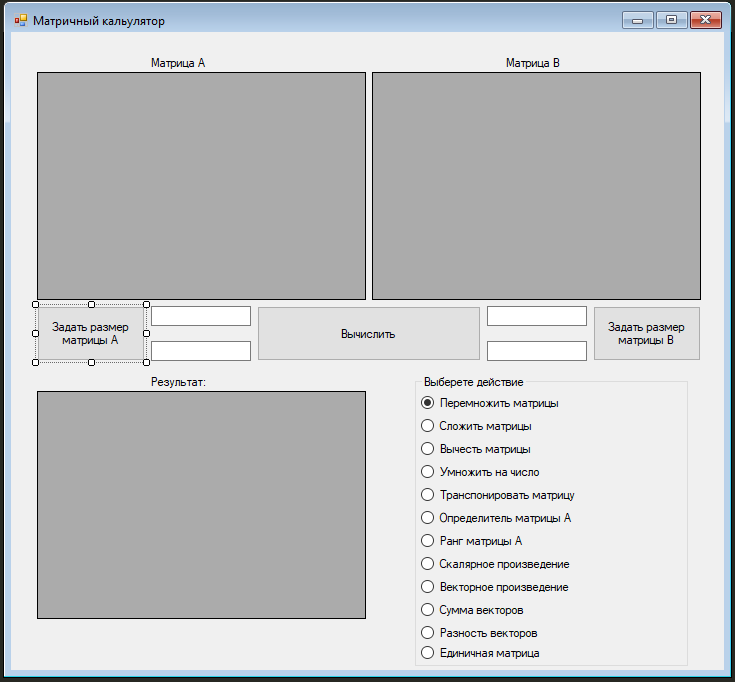
\includegraphics[width = 0.6\textwidth]{images/Task6/FormInConstructor.png}
    \caption{Вид формы в конструкторе}
    \label{fig:FormInConstruct6}
\end{figure}

\subsection{Таблица с описанием переименовнных элементов формы}

Все элементы формы были переименованы и их атрибыты изменены. Проведенные изменения представлены в таблице \ref{tab:label6}

\begin{longtable}[!h]{|l|l|l|}
    \caption{Значения атрибутов элементов в приложении <<Матричный калькулятор>>}
    \label{tab:label6}
    \hline
    \makecell{$\textbf{Описание элементов}$\\ $\textbf{формы}$}& \makecell{$\textbf{Список измененных}$\\ $\textbf{атрибутов}$}& \makecell{$\textbf{Новое значение}$\\ $\textbf{атрибута}$}\\ 
    \hline
    \makecell{Форма}& \makecell{Text}& \makecell{Матричный\\ калькулятор}\\ 
    \hline
    \makecell{Первая надпись (label)}& \makecell{Name}& \makecell{labelA}\\ 
    \hline
    \makecell{Первая надпись (label)}& \makecell{Text}& \makecell{Матрица A}\\ 
    \hline
    \makecell{Вторая надпись (label)}& \makecell{Name}& \makecell{labelB}\\ 
    \hline
    \makecell{Вторая надпись (label)}& \makecell{Text}& \makecell{Матрица B}\\ 
    \hline
    \makecell{Третья надпись (label)}& \makecell{Name}& \makecell{labelRes}\\ 
    \hline
    \makecell{Третья надпись (label)}& \makecell{Text}& \makecell{Результат:}\\ 
    \hline

    \makecell{Первое текстовое\\ поле (textBox)}& \makecell{Name}& \makecell{tbRowAInput}\\ 
    \hline
    \makecell{Второе текстовое\\ поле (textBox)}& \makecell{Name}& \makecell{tbColumnAInput}\\ 
    \hline
    \makecell{Третье текстовое\\ поле (textBox)}& \makecell{Name}& \makecell{tbRowBInput}\\ 
    \hline
    \makecell{Четвёртое текстовое\\ поле (textBox)}& \makecell{Name}& \makecell{tbColumnBInput}\\ 
    \hline

    \makecell{Первая кнопка (button)}& \makecell{Name}& \makecell{btnSizeA}\\ 
    \hline
    \makecell{Первая кнопка (button)}& \makecell{Text}& \makecell{Задать размер\\ матрицы A}\\ 
    \hline
    \makecell{Вторая кнопка (button)}& \makecell{Name}& \makecell{btnSizeB}\\ 
    \hline
    \makecell{Вторая кнопка (button)}& \makecell{Text}& \makecell{Задать размер\\ матрицы B}\\ 
    \hline
    \makecell{Третья кнопка (button)}& \makecell{Name}& \makecell{btnResult}\\ 
    \hline
    \makecell{Третья кнопка (button)}& \makecell{Text}& \makecell{Вычислить}\\ 
    \hline

    \makecell{Первая таблица (dataGridView)}& \makecell{Name}& \makecell{matrixA}\\ 
    \hline
    \makecell{Вторая таблица (dataGridView)}& \makecell{Name}& \makecell{matrixB}\\ 
    \hline
    \makecell{Третья таблица (dataGridView)}& \makecell{Name}& \makecell{matrixResult}\\ 
    \hline

    \makecell{Кнопка выбора 1\\ (radioButton)}& \makecell{Name}& \makecell{rBtnMultMatr}\\ 
    \hline
    \makecell{Кнопка выбора 1\\ (radioButton)}& \makecell{Text}& \makecell{Перемножить\\ матрицы}\\ 
    \hline
    \makecell{Кнопка выбора 2\\ (radioButton)}& \makecell{Name}& \makecell{rBtnSum}\\ 
    \hline
    \makecell{Кнопка выбора 2\\ (radioButton)}& \makecell{Text}& \makecell{Сложить\\ матрицы}\\ 
    \hline
    \makecell{Кнопка выбора 3\\ (radioButton)}& \makecell{Name}& \makecell{rBtnSubstract}\\ 
    \hline
    \makecell{Кнопка выбора 3\\ (radioButton)}& \makecell{Text}& \makecell{Вычесть\\ матрицы}\\ 
    \hline
    \makecell{Кнопка выбора 4\\ (radioButton)}& \makecell{Name}& \makecell{rBtnMultNum}\\ 
    \hline
    \makecell{Кнопка выбора 4\\ (radioButton)}& \makecell{Text}& \makecell{Умножить\\ на число}\\ 
    \hline
    \makecell{Кнопка выбора 5\\ (radioButton)}& \makecell{Name}& \makecell{rBtnTransposition}\\ 
    \hline
    \makecell{Кнопка выбора 5\\ (radioButton)}& \makecell{Text}& \makecell{Транспонировать\\ матрицу}\\ 
    \hline
    \makecell{Кнопка выбора 6\\ (radioButton)}& \makecell{Name}& \makecell{rBtnDetermA}\\ 
    \hline
    \makecell{Кнопка выбора 6\\ (radioButton)}& \makecell{Text}& \makecell{Определитель\\ матрицы A}\\ 
    \hline
    \makecell{Кнопка выбора 7\\ (radioButton)}& \makecell{Name}& \makecell{rBtnRankA}\\ 
    \hline
    \makecell{Кнопка выбора 7\\ (radioButton)}& \makecell{Text}& \makecell{Ранг\\ матрицы A}\\ 
    \hline
    \makecell{Кнопка выбора 8\\ (radioButton)}& \makecell{Name}& \makecell{rBtnScalar}\\ 
    \hline
    \makecell{Кнопка выбора 8\\ (radioButton)}& \makecell{Text}& \makecell{Скалярное\\ произведение}\\ 
    \hline
    \makecell{Кнопка выбора 9\\ (radioButton)}& \makecell{Name}& \makecell{rBtnVector}\\ 
    \hline
    \makecell{Кнопка выбора 9\\ (radioButton)}& \makecell{Text}& \makecell{Векторное\\ произведение}\\ 
    \hline
    \makecell{Кнопка выбора 10\\ (radioButton)}& \makecell{Name}& \makecell{rBtnSumVec}\\ 
    \hline
    \makecell{Кнопка выбора 10\\ (radioButton)}& \makecell{Text}& \makecell{Сумма\\ векторов}\\ 
    \hline
    \makecell{Кнопка выбора 11\\ (radioButton)}& \makecell{Name}& \makecell{rBtnSubVec}\\ 
    \hline
    \makecell{Кнопка выбора 11\\ (radioButton)}& \makecell{Text}& \makecell{Разность\\ векторов}\\ 
    \hline
    \makecell{Кнопка выбора 12\\ (radioButton)}& \makecell{Name}& \makecell{rBtnUnitMatrix}\\ 
    \hline
    \makecell{Кнопка выбора 12\\ (radioButton)}& \makecell{Text}& \makecell{Единичная\\ матрица}\\ 
    \hline

    \makecell{groupBox}& \makecell{Name}& \makecell{grChoose}\\ 
    \hline
    \makecell{groupBox}& \makecell{Text}& \makecell{Выбор\\ действия}\\ 
    \hline

    \makecell{Обработчик ошибок 1\\ (errorProvider)}& \makecell{Name}& \makecell{erPrSizeA}\\ 
    \hline
    \makecell{Обработчик ошибок 2\\ (errorProvider)}& \makecell{Name}& \makecell{erPrSizeB}\\ 
    \hline
    \makecell{Обработчик ошибок 3\\ (errorProvider)}& \makecell{Name}& \makecell{erPrResult}\\ 
    \hline
\end{longtable}

\subsection{Примеры работы}

При запуске приложения на экране появляется окно (\ref{fig:StartForm6}).

\newpage

\begin{figure}[!h]
    \centering
    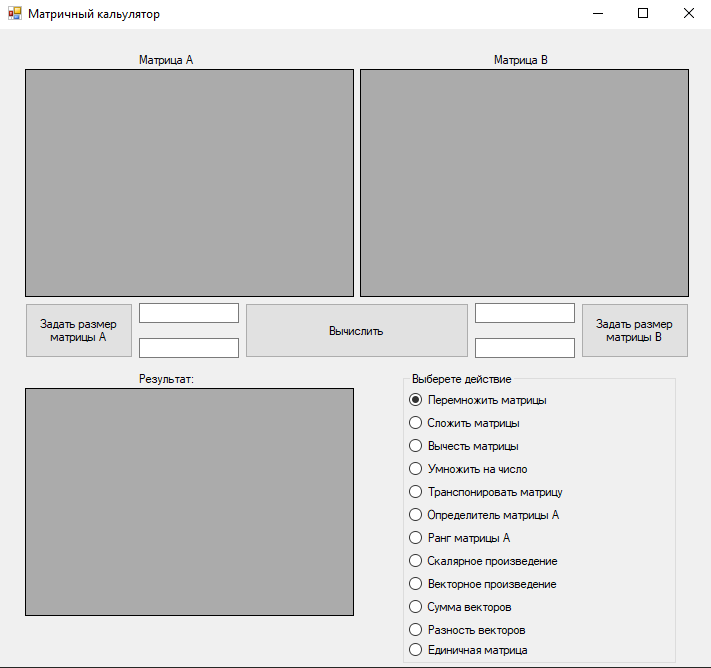
\includegraphics[width = 0.5\textwidth]{images/Task6/Start.png}
    \caption{Запуск приложения}
    \label{fig:StartForm6}
\end{figure}

При запуске с корректными данными, при нажатии на кнопку <<Вычислить>> c выбранным действием <<Сложить матрицы>> происходит (\ref{fig:WorkForm6}):

\begin{figure}[!h]
    \centering
    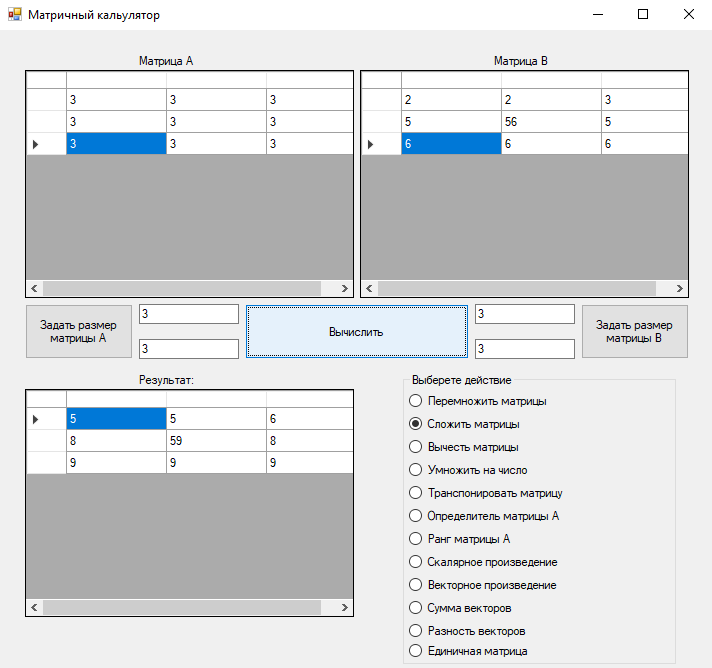
\includegraphics[width = 0.6\textwidth]{images/Task6/WorkSum.png}
    \caption{Запуск с корректными данными}
    \label{fig:WorkForm6}
\end{figure}

При запуске с некорректными данными,, при нажатии на кнопку <<Вычислить>> c выбранным действием <<Сложить матрицы>> происходит (\ref{fig:BadInputNotIntForm6}):

\begin{figure}[!h]
    \centering
    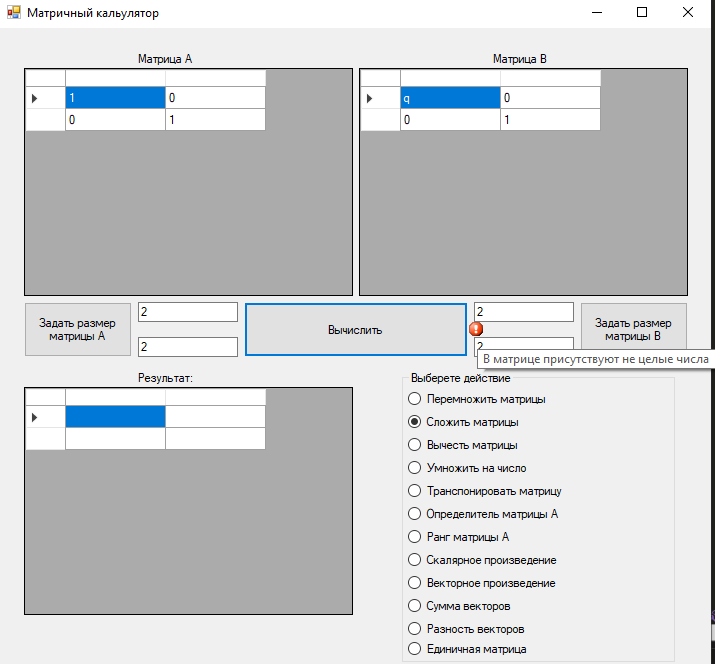
\includegraphics[width = 0.6\textwidth]{images/Task6/BadInputSumMatrix.png}
    \caption{Запуск с некорректными данными}
    \label{fig:BadInputNotIntForm6}
\end{figure}

\subsection{Примеры кода}

Функция умножения матрицы $A$ на число $num$

\begin{minted}{c++}
		// умножение матрицы A на число num
		void MultNum(int row, int column, int num) {
			int a;
			bool check;
			for (int i = 0; i < row; i++) {
				for (int j = 0; j < column; j++) {
					// Проверка на не целое число
					check = Int32::TryParse(System::Convert::ToString(matrixA->Rows[i]->Cells[j]->Value), a);
					if (!check) {
						throw gcnew FormatException("В матрице присутствуют не целые числа");
					}
					// Умножение на число
					matrixResult->Rows[i]->Cells[j]->Value = a * num;
				}
			}
		}
\end{minted}

Другие фрагменты кода расположены в приложении \ref{app:task6}. Полный код программы приведен в приложении \ref{app:zip}
